\chapter{Cơ sở lý thuyết và các nghiên cứu liên quan}
\label{ch:co-so-ly-thuyet}

Chương này trình bày cơ sở phương pháp luận học máy và tổng quan y văn cho bài toán dự đoán mức độ triệu chứng trầm cảm từ dữ liệu sinh lý dạng bảng, bao gồm: (1) cấu trúc thang đo PHQ-9; (2) hai đặc thù lớn của dữ liệu y tế dạng bảng gồm mất cân bằng lớp và chồng lấn phân phối đặc trưng; (3) các trường phái mô hình hóa gồm phân loại phẳng, phân loại phân cấp kết hợp lý thuyết quyết định Bayes, và phân loại thứ bậc; (4) tổng hợp và phân tích các công trình nghiên cứu liên quan.

\section{Thang đo PHQ-9 và bài toán lượng hóa mức độ trầm cảm}
\label{sec:thang-do-phq9}

Thang đo Sức khỏe Bệnh nhân 9 mục (Patient Health Questionnaire-9 -- PHQ-9) là công cụ sàng lọc tâm thần tự báo cáo được chuẩn hóa quốc tế do Kroenke và cộng sự phát triển \cite{kroenke2001phq, spitzer1999validation}. Bảng hỏi gồm 9 mục đánh giá tần suất xuất hiện các triệu chứng trong 2 tuần gần nhất theo tiêu chuẩn DSM-IV, mỗi mục được chấm điểm từ 0 đến 3 (0: hoàn toàn không; 1: vài ngày; 2: hơn một nửa số ngày; 3: gần như mỗi ngày).

\begin{figure}[htbp]{Thang đo PHQ-9 (0--27 điểm), 5 khoảng mức độ triệu chứng và ánh xạ sang không gian 3 nhóm $T_3$.}
\centering
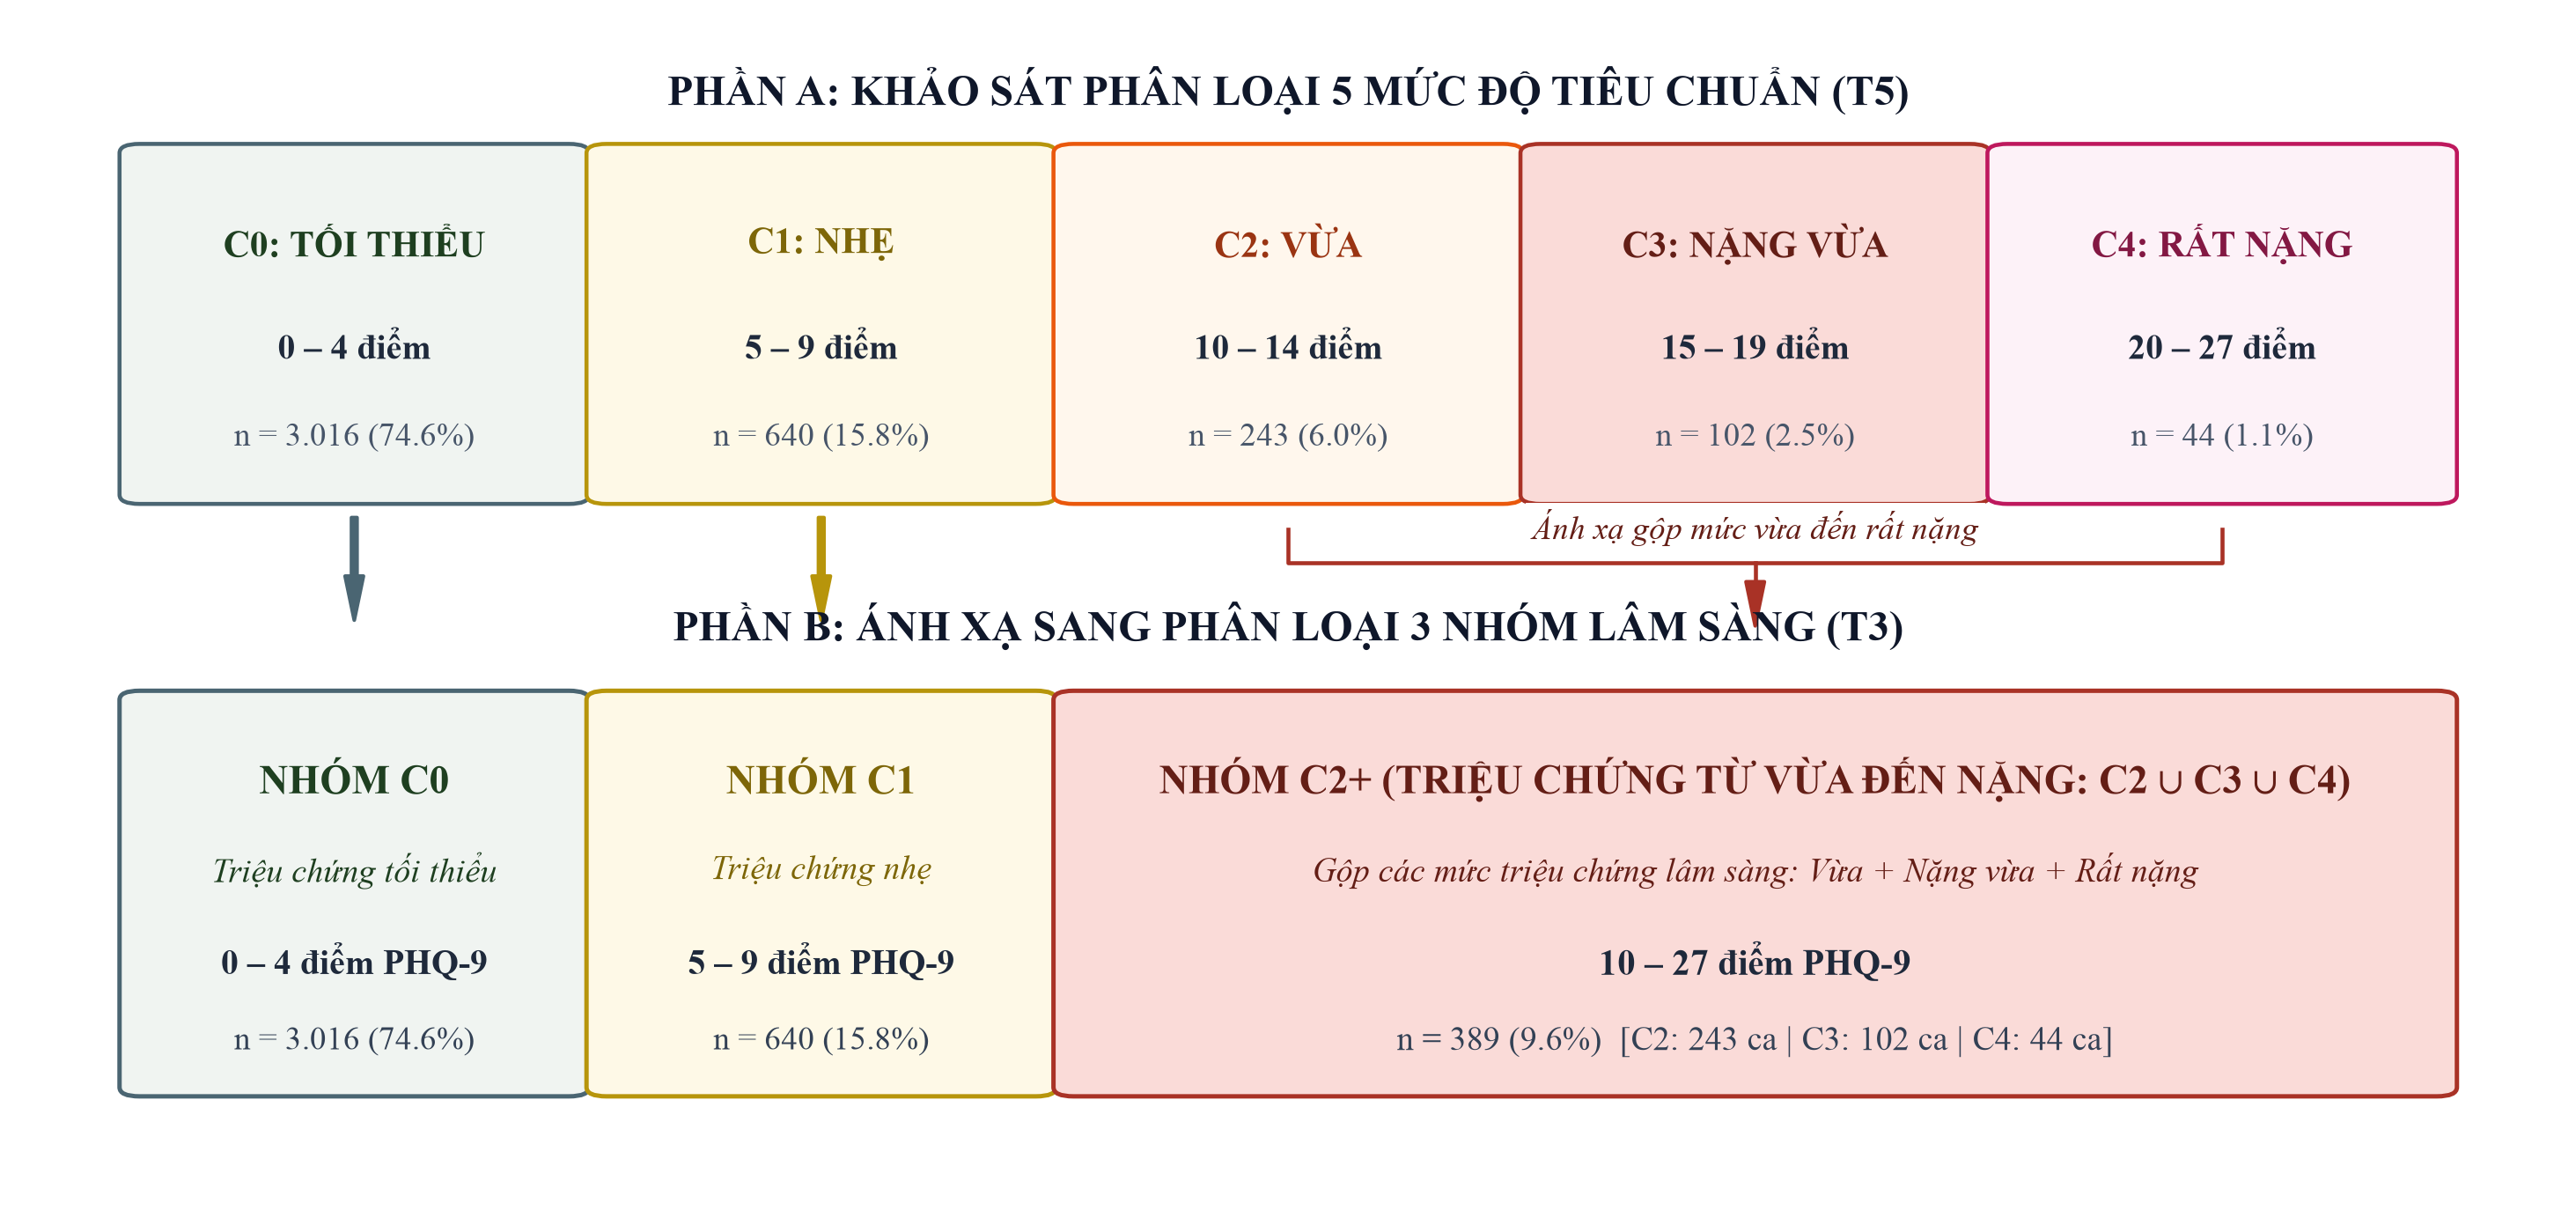
\includegraphics[width=0.92\textwidth]{figures/fig2_phq9_tiers.png}
\label{fig:phq9-tiers}
\end{figure}

Tổng điểm $s = \sum_{j=1}^9 \text{DPQ}_j \in [0, 27]$ được phân chia thành 5 khoảng mức độ tiêu chuẩn trong dịch tễ học như minh họa trong Hình \ref{fig:phq9-tiers}A:
\begin{itemize}
    \item $s \in [0, 4]$ ($C_0$ -- Tối thiểu): phản ánh trạng thái tâm lý ổn định, không có triệu chứng đáng kể.
    \item $s \in [5, 9]$ ($C_1$ -- Nhẹ): có triệu chứng nhẹ, thường được khuyến nghị theo dõi hoặc can thiệp lối sống.
    \item $s \in [10, 14]$ ($C_2$ -- Vừa): mức độ vừa, là ngưỡng khuyến cáo cần thăm khám lâm sàng.
    \item $s \in [15, 19]$ ($C_3$ -- Nặng vừa): triệu chứng nặng vừa, cần can thiệp tâm lý hoặc dùng thuốc.
    \item $s \in [20, 27]$ ($C_4$ -- Nặng): mức độ nặng nhất, có nguy cơ cao về hành vi tự hủy hoại bản thân.
\end{itemize}

Trong đề tài DepSev-ML, bên cạnh bài toán 5 mức gốc ($T_5$), bài toán còn được khảo sát trên không gian 3 nhóm ($T_3$, Hình \ref{fig:phq9-tiers}B), trong đó nhóm $C_2^+$ đại diện cho toàn bộ các đối tượng có điểm PHQ-9 $\ge 10$ ($C_2 \cup C_3 \cup C_4$), gọi là nhóm Nặng theo quy ước nghiên cứu. Việc phân tầng 3 nhóm này giúp liên kết trực tiếp kết quả mô hình với các định hướng can thiệp y tế dự phòng trong cộng đồng.

\section{Đặc thù và thách thức của dữ liệu y tế dạng bảng}
\label{sec:dac-thu-du-lieu}

Dữ liệu khảo sát sức khỏe cộng đồng NHANES mang hai đặc thù lớn ảnh hưởng trực tiếp đến hiệu năng của các thuật toán học máy:

\begin{figure}[htbp]{Hai thách thức đặc thù của dữ liệu y tế dạng bảng: Mất cân bằng lớp và Chồng lấn phân phối sinh lý.}
\centering
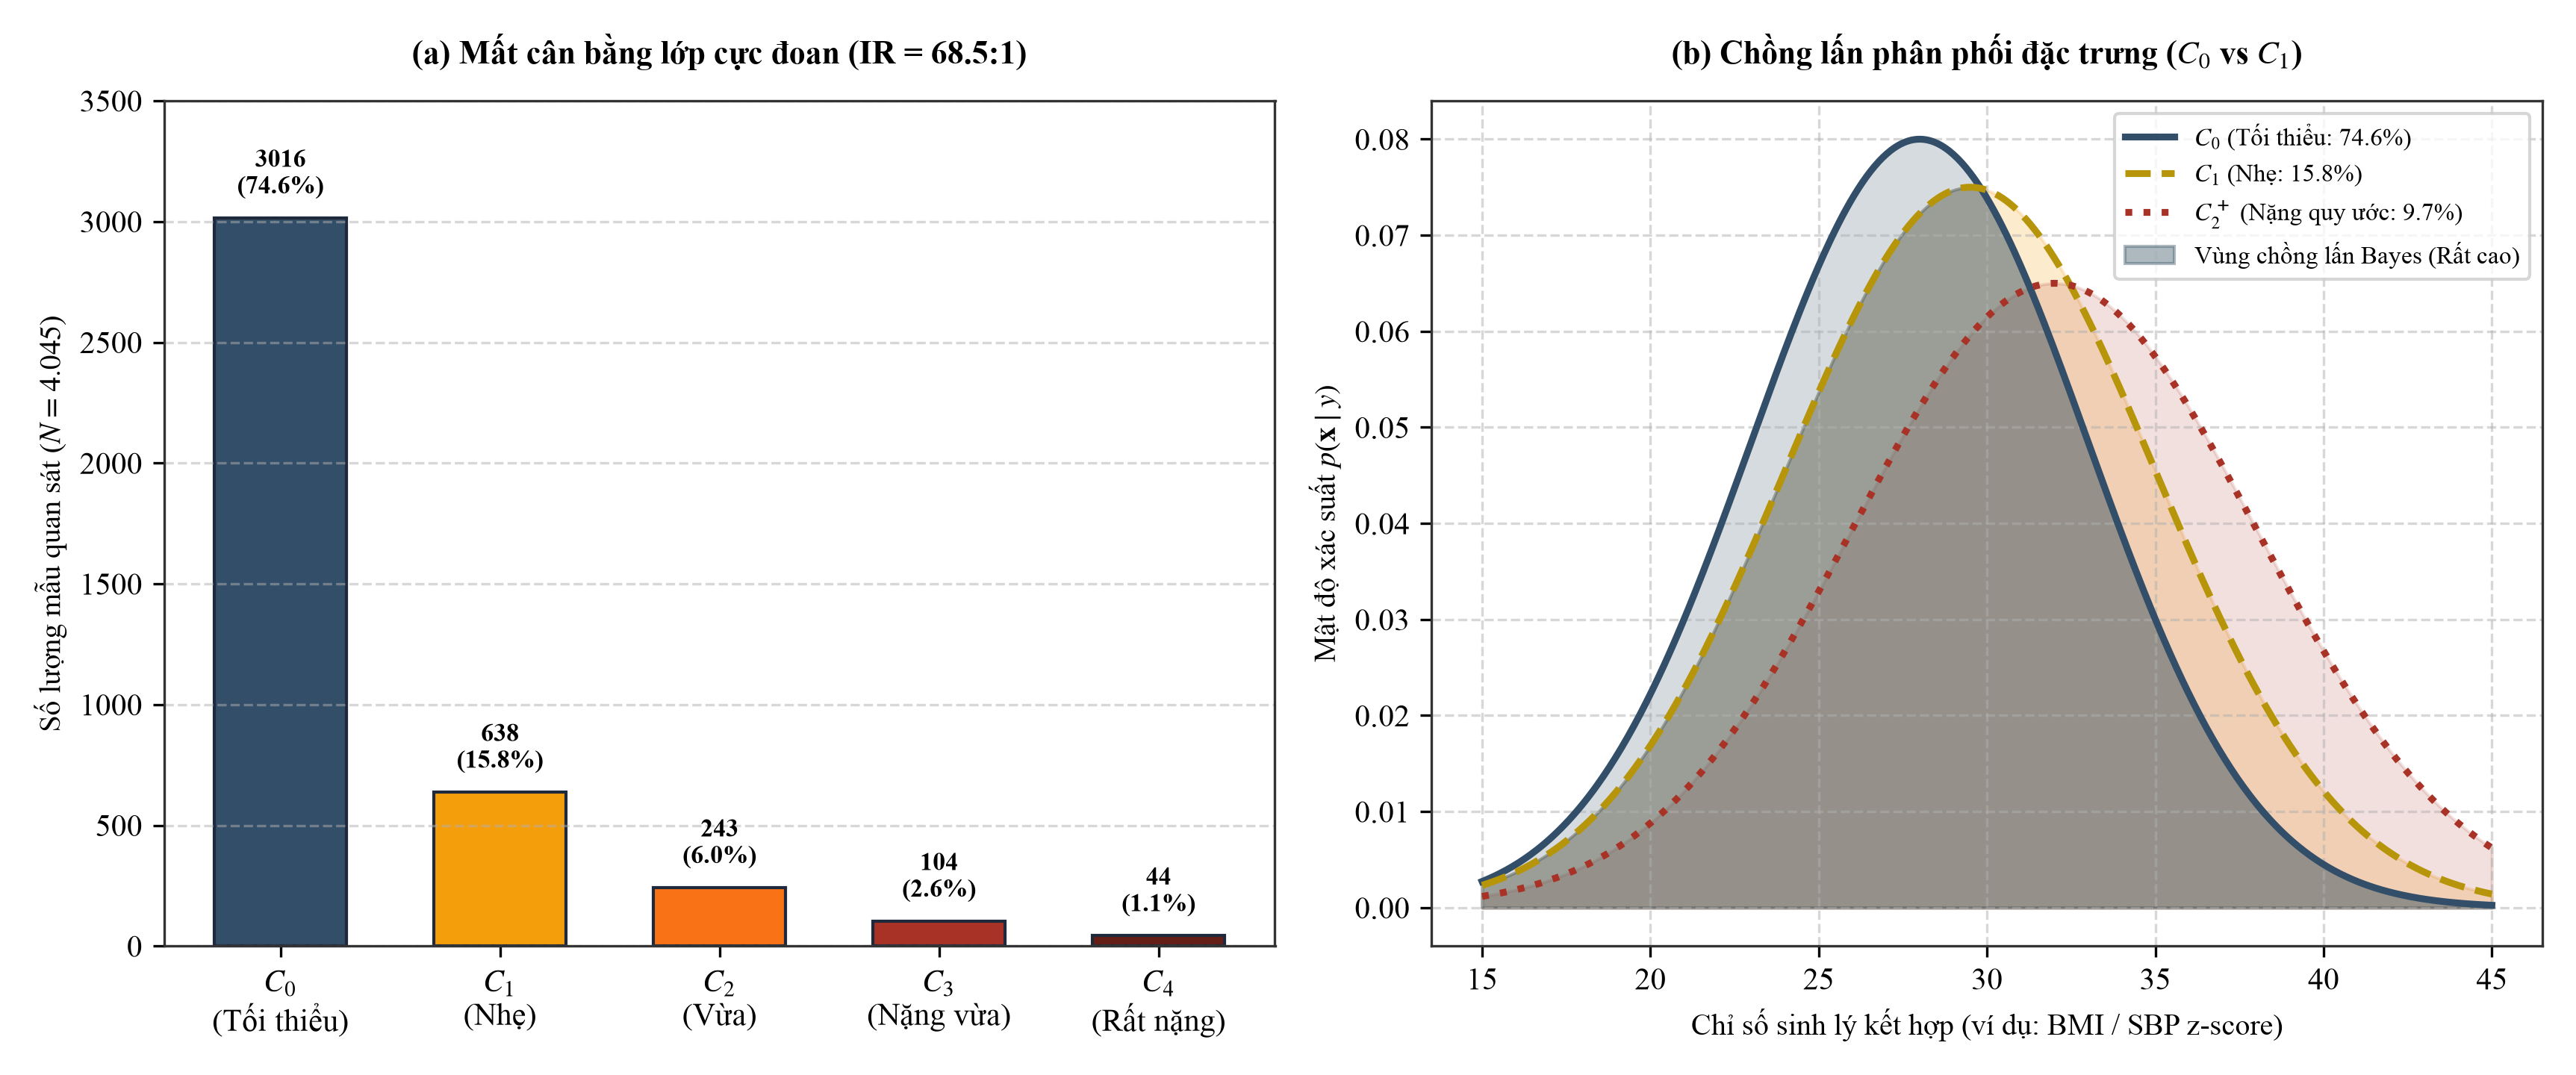
\includegraphics[width=0.92\textwidth]{figures/fig2_imbalance_overlap.png}
\label{fig:imbalance-overlap}
\end{figure}

\begin{enumerate}
    \item \textit{Mất cân bằng lớp cực đoan (Severe Class Imbalance):} Do phần lớn dân số trong cộng đồng khỏe mạnh, lớp $C_0$ chiếm tới 76.14\% tổng mẫu, trong khi nhóm có triệu chứng từ vừa đến nặng ($C_2^+$) chỉ chiếm 7.37\%, và lớp nặng nhất ($C_4$) chỉ chiếm 1.09\% (Hình \ref{fig:imbalance-overlap}A). Tỷ lệ mất cân bằng vượt quá 10:1 khiến các mô hình học máy thông thường dễ rơi vào bẫy dự đoán toàn bộ về lớp đa số, đạt độ chính xác bề nổi cao nhưng mất khả năng nhận diện các ca bệnh thực tế.
    \item \textit{Chồng lấn phân phối đặc trưng (Feature Overlap):} Trầm cảm là hội chứng tâm thần kinh phức tạp, không có chỉ dấu sinh học ngoại vi mang tính quyết định tuyệt đối trong máu. Các chỉ số như huyết áp, chỉ số khối cơ thể, bạch cầu hay cholesterol giữa các nhóm triệu chứng có độ phân tán lớn và chồng lấn rõ rệt trong không gian đặc trưng (Hình \ref{fig:imbalance-overlap}B), khiến các ranh giới phân tách trở nên mờ nhạt.
\end{enumerate}

\section{Các trường phái mô hình hóa trong bài toán phân loại thứ bậc}
\label{sec:truong-phai-mo-hinh}

Để giải quyết bài toán phân loại triệu chứng trầm cảm trên không gian 3 nhóm ($T_3$), nghiên cứu phân loại các phương pháp tiếp cận thành 4 trường phái như minh họa trong Hình \ref{fig:modeling-paradigms}.

\begin{figure}[htbp]{Sơ đồ so sánh 4 trường phái mô hình hóa được khảo sát trong nghiên cứu DepSev-ML.}
\centering
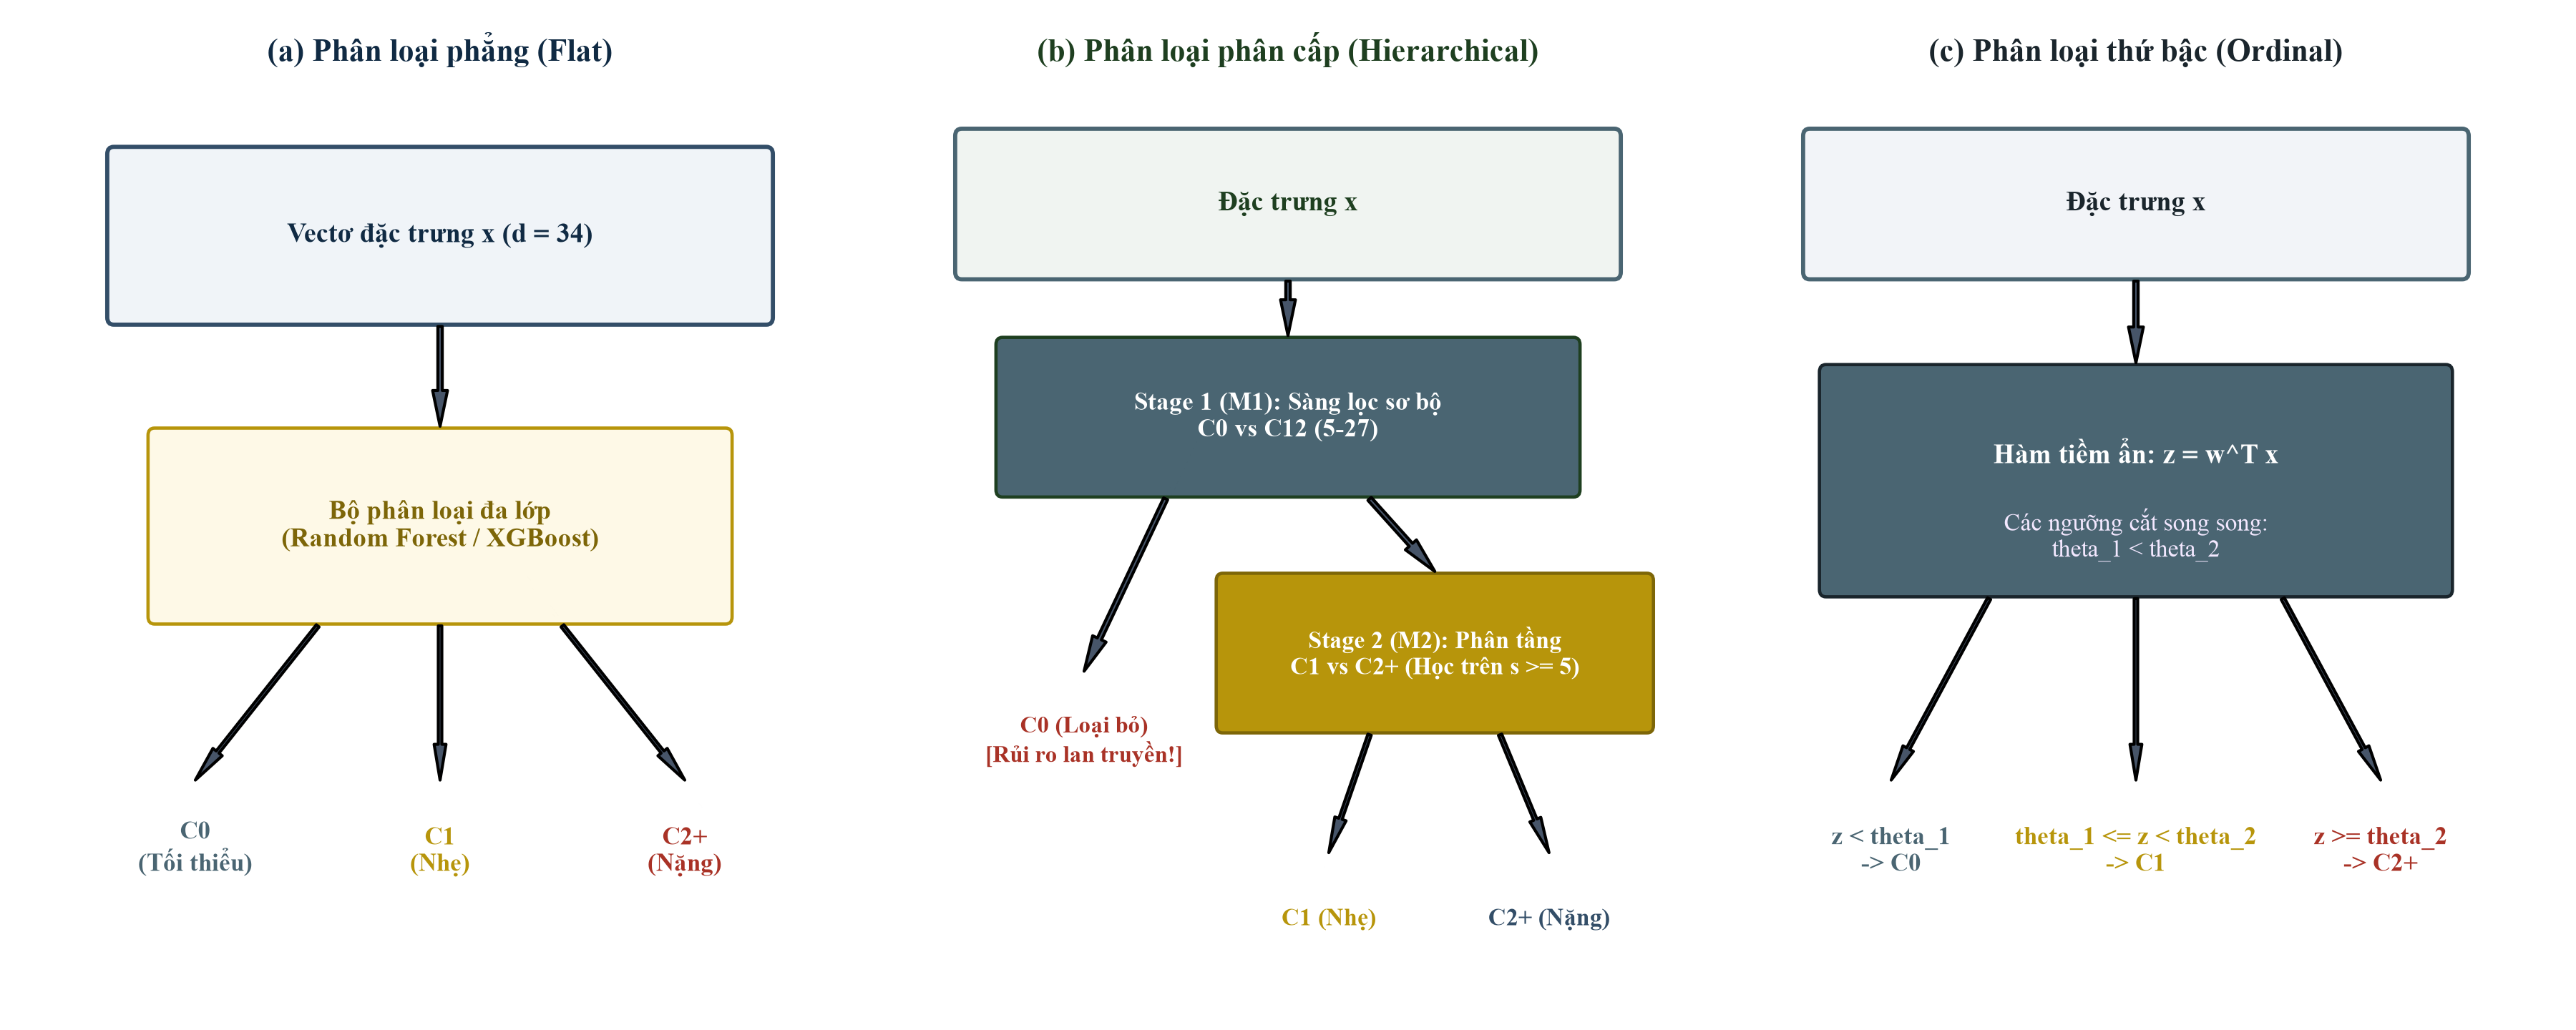
\includegraphics[width=0.95\textwidth]{figures/fig2_modeling_paradigms.png}
\label{fig:modeling-paradigms}
\end{figure}

\subsection{Trường phái phân loại phẳng (Flat Classification)}
\label{subsec:flat-paradigm}

Mô hình phân loại phẳng coi $K$ lớp là các nhãn danh nghĩa độc lập, bỏ qua trật tự thứ bậc giữa các mức độ triệu chứng. Mô hình nhận vectơ đầu vào $\mathbf{x} \in \mathbb{R}^d$ và dự đoán trực tiếp nhãn $\hat{y} \in \{C_0, C_1, C_2^+\}$. 

Trong nghiên cứu này, thuật toán Random Forest \cite{breiman2001random} được lựa chọn làm mô hình phẳng cơ sở (Backbone Baseline). Random Forest kết hợp nhiều cây quyết định độc lập qua kỹ thuật Bootstrap Sampling và ngẫu nhiên hóa không gian đặc trưng. Dựa trên kết quả thực nghiệm kiểm định chéo lồng nhau trên 34 đặc trưng ($F_4$), Random Forest đạt điểm Macro-F1 cao nhất ($0.2755 \pm 0.0152$) trong số các thuật toán cơ sở và thể hiện tính ổn định cao trước hiện tượng quá khớp trên dữ liệu dạng bảng.

\subsection{Trường phái phân loại phân cấp (Hierarchical Classification)}
\label{subsec:hierarchical-paradigm}

Phương pháp phân loại phân cấp chia bài toán 3 nhóm thành hai giai đoạn nối tiếp: Giai đoạn 1 sàng lọc người có triệu chứng ($C_0$ so với $C_{12} = C_1 \cup C_2^+$); Giai đoạn 2 phân định mức độ nghiêm trọng ($C_1$ so với $C_2^+$). Hai cơ chế định tuyến được thử nghiệm gồm:
\begin{itemize}
    \item \textit{Định tuyến cứng (Hard Routing):} Nếu Giai đoạn 1 dự đoán mẫu là $C_0$, mẫu đó lập tức kết thúc luồng xử lý. Cơ chế này dẫn đến hiện tượng tắc nghẽn sai số một chiều: nếu một ca nặng $C_2^+$ bị Giai đoạn 1 gán nhầm thành $C_0$, sai số này không thể khắc phục ở Giai đoạn 2.
    \item \textit{Định tuyến mềm (Soft Routing):} Cả hai mô hình đều xuất ra vectơ xác suất liên tục. Xác suất hậu nghiệm toàn thể $\hat{P}(C_k \mid \mathbf{x})$ được kết hợp theo công thức xác suất toàn phần, bảo toàn thông tin định lượng và loại bỏ hiện tượng tắc nghẽn một chiều.
\end{itemize}

\subsection{Lý thuyết quyết định nhạy chi phí Bayes (Bayes Cost-Sensitive Decision)}
\label{subsec:cost-sensitive-paradigm}

Trong sàng lọc y tế, sai lầm bỏ sót một ca bệnh nặng ($C_2^+ \to C_0$) gây nguy hiểm lâm sàng lớn hơn nhiều so với một ca báo động nhầm ($C_0 \to C_2^+$). Lý thuyết quyết định Bayes \cite{elkan2001foundations} cung cấp cơ sở toán học để tối ưu quyết định dưới sự bất cân xứng này.

Cho ma trận chi phí phạt $\mathbf{C} \in \mathbb{R}^{K \times K}$, trong đó $\mathbf{C}(i, j)$ là chi phí tổn thất khi nhãn thực tế là $i$ nhưng dự đoán là $j$ (với $\mathbf{C}(i, i) = 0$). Rủi ro kỳ vọng được tính theo:
\begin{equation}
    R(j \mid \mathbf{x}) = \sum_{i=0}^{K-1} \hat{P}(C_i \mid \mathbf{x}) \cdot \mathbf{C}(i, j)
\end{equation}
Quy tắc quyết định Bayes lựa chọn nhãn tối ưu $\hat{y}^* = \arg\min_j R(j \mid \mathbf{x})$ nhằm tối thiểu hóa tổn thất kỳ vọng toàn cục. Bằng cách gán trọng số phạt lớn cho phần tử $\mathbf{C}(2, 0)$ (nhãn thực là $C_2^+$, dự đoán thành $C_0$), mô hình chủ động dịch chuyển ranh giới quyết định để bảo vệ các ca nặng.

\subsection{Phương pháp phân loại thứ bậc (Ordinal Classification)}
\label{subsec:ordinal-paradigm}

Do các mức độ triệu chứng PHQ-9 có tính thứ tự tự nhiên ($C_0 < C_1 < C_2^+$), phân loại thứ bậc khai thác cấu trúc trật tự này để hạn chế các sai số nhảy bậc lớn \cite{mccullagh1980regression, frank2001simple}:
\begin{itemize}
    \item \textit{Mô hình Ordinal Logistic Regression (OLR):} Giả định tồn tại một biến tiềm ẩn tuyến tính $z = \mathbf{w}^T \mathbf{x}$ cùng các ngưỡng cắt đơn điệu $\theta_1 < \theta_2$. Mô hình sử dụng chung vectơ trọng số $\mathbf{w}$ cho tất cả các ranh giới, bảo đảm các siêu phẳng quyết định song song và không bao giờ cắt nhau.
    \item \textit{Phân loại nhị phân tích lũy (Cumulative Binary Classification -- CBC):} Huấn luyện các bộ phân loại nhị phân độc lập để dự đoán biến cố tích lũy $P(Y \ge k \mid \mathbf{x})$. Tuy nhiên, phương pháp này tiềm ẩn nguy cơ vi phạm tính đơn điệu xác suất khi xuất hiện $P(Y \ge 2) > P(Y \ge 1)$ trên một số mẫu thực tế.
\end{itemize}

\section{Tổng quan các nghiên cứu liên quan}
\label{sec:nghien-cuu-lien-quan}

Bảng \ref{tab:related-works} tổng hợp các công trình tiêu biểu áp dụng học máy trên dữ liệu khảo sát sức khỏe NHANES để dự đoán triệu chứng trầm cảm.

\begin{table}[htbp]{Tổng hợp so sánh các nghiên cứu liên quan về dự đoán trầm cảm từ dữ liệu y tế.}
\centering
\small
\setlength{\tabcolsep}{4pt}
\label{tab:related-works}
\begin{tabularx}{\textwidth}{p{3.0cm} p{2.2cm} p{3.4cm} X}
\toprule
\textbf{Nghiên cứu} & \textbf{Dữ liệu} & \textbf{Phương pháp} & \textbf{Kết quả \& Giới hạn chính} \\
\midrule
Pratt và cs. (2014) \cite{pratt2014depression} & NHANES 2009--2012 & Hồi quy logistic, dịch tễ & Đánh giá tỷ lệ mắc và yếu tố nguy cơ dân số; không xây dựng mô hình học máy dự đoán. \\
\midrule
Patel và cs. (2016) \cite{patel2016systematic} [UNVERIFIED] & NHANES đa chu kỳ & Logistic Regression, Decision Tree & Khảo sát yếu tố nguy cơ; chỉ dừng ở bài toán nhị phân ($s \ge 10$), chưa phân tầng đa mức. \\
\midrule
Dipnall và cs. (2016) \cite{dipnall2016fusing} & NHANES 2009--2010 & Khai phá dữ liệu, GLM & Kết hợp dấu ấn sinh học cận lâm sàng; chỉ phân loại nhị phân, chưa khảo sát đa mức $T_3 \to T_5$. \\
\midrule
Zhang và cs. (2020) \cite{zhang2020machine} [UNVERIFIED] & Khảo sát dạng bảng & Random Forest, XGBoost phẳng & So sánh thuật toán dạng bảng; phân loại phẳng, chưa tối ưu chi phí cho các ca nặng. \\
\midrule
DepSev-ML (Đề tài) & NHANES 3 chu kỳ & RF, Phân cấp mềm, Bayes Risk, OLR & Khảo sát đa mức $T_2 \to T_5$; giảm 48.33\% ca nặng bị bỏ sót với chi phí Bayes; kiểm định ngoại suy thời gian. \\
\bottomrule
\end{tabularx}
\end{table}

Qua khảo sát y văn, có thể nhận thấy đa số các công trình trước đây chỉ tập trung vào bài toán nhị phân đơn giản ($s \ge 10$). Rất ít nghiên cứu phân tích sự suy giảm hiệu năng khi phân tầng đa mức, cũng như thiếu sự đánh giá so sánh có hệ thống giữa các trường phái phân cấp, nhạy chi phí Bayes và phân loại thứ bậc. Đề tài DepSev-ML được thiết kế để giải quyết trọn vẹn những khoảng trống nghiên cứu này.
